% The Adafruit DRV8833 motor driver breakout, seen from above with its
% headers soldered on, and the five connections the mini rig uses. Pin and
% terminal positions are taken from Adafruit's board file
% (github.com/adafruit/Adafruit-DRV8833-Motor-Driver-Breakout-PCB), in mm.
\documentclass[border=2pt]{standalone}
\usepackage[svgnames]{xcolor}
\usepackage{tikz}
\definecolor{signal}{RGB}{245,195,0}
\definecolor{pcb}{RGB}{28,58,135}

\begin{document}
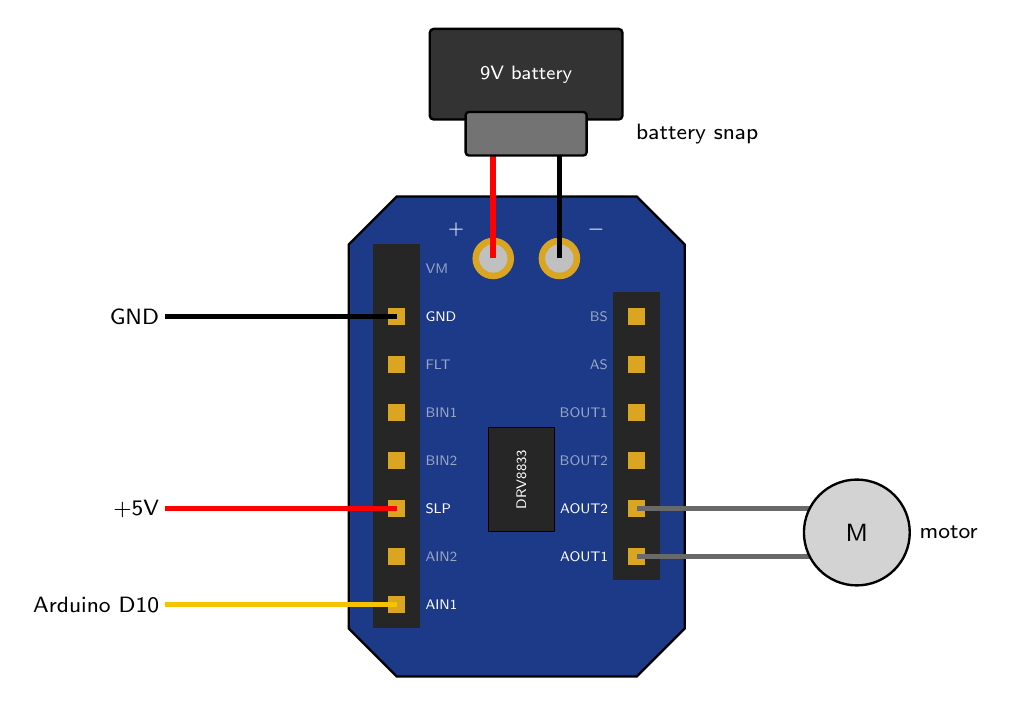
\begin{tikzpicture}[
    x=.24cm, y=.24cm,
    pinlabel/.style={font=\sffamily\tiny, text=white, inner sep=1pt},
    unused/.style={pinlabel, text=white!55!pcb},
    wire/.style={line width=.7mm, rounded corners=.6mm},
    label/.style={font=\sffamily\footnotesize, inner sep=2pt},
]
    %% the board, with its chamfered corners
    \filldraw[fill=pcb, draw=black, line width=.3mm]
        (0.254, 24.13) -- (12.954, 24.13) -- (15.494, 21.59)
        -- (15.494, 1.27) -- (12.954, -1.27) -- (0.254, -1.27)
        -- (-2.286, 1.27) -- (-2.286, 21.59) -- cycle;
    %% the DRV8833 chip in the middle
    \filldraw[fill=black!85] (5.1, 6.4) rectangle (8.6, 11.9);
    \node[pinlabel, rotate=90] at (6.85, 9.15) {DRV8833};

    %% the soldered header strips: black plastic, with gold pins
    \fill[black!85] (-0.98, 1.27) rectangle (1.49, 21.59);
    \fill[black!85] (11.72, 3.81) rectangle (14.19, 19.05);
    \foreach \y in {2.54, 5.08, ..., 20.32}
        \fill[Goldenrod] (0.254, \y) +(-.45, -.45) rectangle +(.45, .45);
    \foreach \y in {5.08, 7.62, ..., 17.78}
        \fill[Goldenrod] (12.954, \y) +(-.45, -.45) rectangle +(.45, .45);

    %% pin names, as on the silkscreen; the ones we use are bright
    \foreach \y/\name/\style in {20.32/VM/unused, 17.78/GND/pinlabel,
            15.24/FLT/unused, 12.7/BIN1/unused, 10.16/BIN2/unused,
            7.62/SLP/pinlabel, 5.08/AIN2/unused, 2.54/AIN1/pinlabel}
        \node[\style, anchor=west] at (1.6, \y) {\name};
    \foreach \y/\name/\style in {17.78/BS/unused, 15.24/AS/unused,
            12.7/BOUT1/unused, 10.16/BOUT2/unused,
            7.62/AOUT2/pinlabel, 5.08/AOUT1/pinlabel}
        \node[\style, anchor=east] at (11.6, \y) {\name};

    %% the motor power pads, + on the left, with the battery snap's leads
    %% soldered in
    \foreach \x in {5.36, 8.86}{
        \fill[Goldenrod] (\x, 20.85) circle (1.1);
        \fill[Silver] (\x, 20.85) circle (.75);
    }
    \node[pinlabel, font=\sffamily\scriptsize] at (3.4, 22.4) {+};
    \node[pinlabel, font=\sffamily\scriptsize] at (10.8, 22.4) {$-$};

    %% from the Arduino and the breadboard
    \draw[wire, draw=signal] (0.254, 2.54) -- (-12, 2.54);
    \node[label, anchor=east] at (-12, 2.54) {Arduino D10};
    \draw[wire, draw=Red] (0.254, 7.62) -- (-12, 7.62);
    \node[label, anchor=east] at (-12, 7.62) {+5V};
    \draw[wire, draw=black] (0.254, 17.78) -- (-12, 17.78);
    \node[label, anchor=east] at (-12, 17.78) {GND};

    %% the 9V battery, clipped onto the battery snap
    \draw[wire, draw=Red] (5.36, 20.85) -- (5.36, 26.5);
    \draw[wire, draw=black] (8.86, 20.85) -- (8.86, 26.5);
    \filldraw[fill=black!80, draw=black, line width=.3mm, rounded corners=.5mm]
        (2, 28.2) rectangle (12.2, 33);
    \node[pinlabel, font=\sffamily\scriptsize] at (7.1, 30.6) {9V battery};
    \filldraw[fill=black!55, draw=black, line width=.3mm, rounded corners=.4mm]
        (3.9, 26.3) rectangle (10.3, 28.6);
    \node[label, anchor=west] at (12.6, 27.45) {battery snap};

    %% the motor, on the A outputs
    \draw[wire, draw=DimGray] (12.954, 5.08) -- (23, 5.08);
    \draw[wire, draw=DimGray] (12.954, 7.62) -- (23, 7.62);
    \filldraw[fill=LightGray, draw=black, line width=.3mm] (24.6, 6.35)
        circle (2.8);
    \node[font=\sffamily\small] at (24.6, 6.35) {M};
    \node[label, anchor=west] at (27.6, 6.35) {motor};
\end{tikzpicture}
\end{document}
